\documentclass{standalone}

\usepackage{tikz}
\usepackage{tikzpeople}

\newcommand{\KGen}{\ensuremath{\mathsf{KeyGen}}}
\newcommand{\Enc}{\ensuremath{\mathsf{Enc}}}
\newcommand{\Dec}{\ensuremath{\mathsf{Dec}}}

\begin{document}

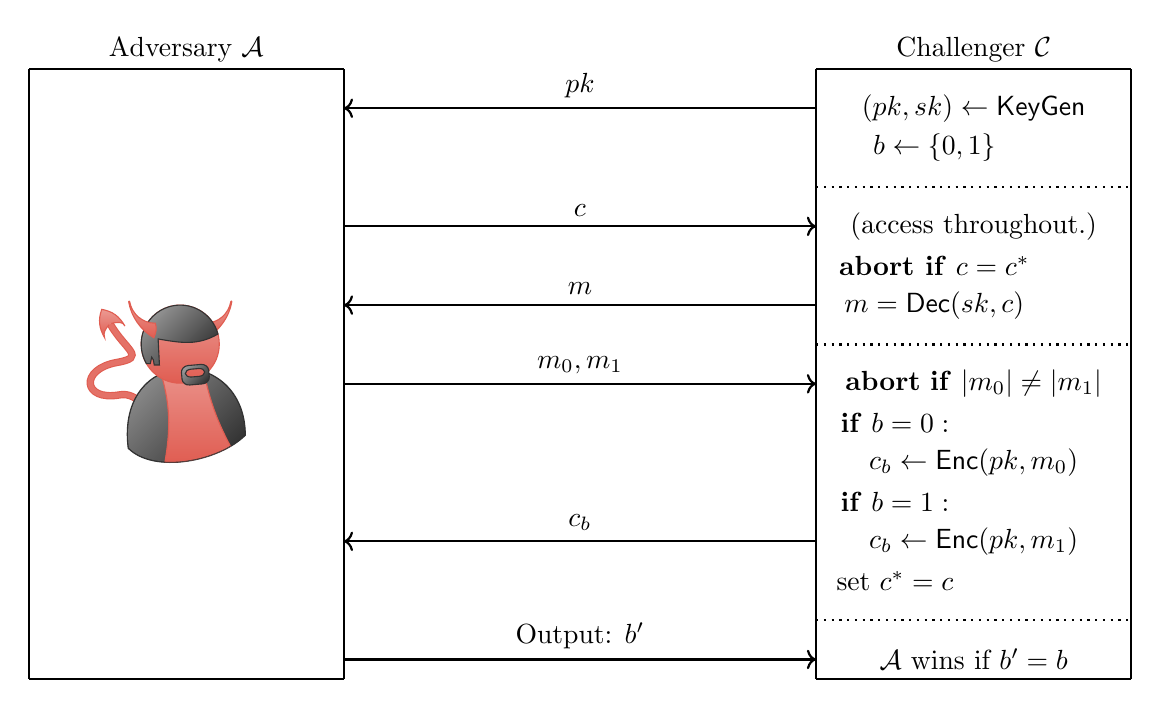
\begin{tikzpicture}

\node[] (lblAdv) at (2,5.25) {Adversary $\mathcal{A}$};
\draw[-,thick] (0,-2.75)--(4,-2.75);
\draw[-,thick] (4,-2.75)--(4,5);
\draw[-,thick] (4,5)--(0,5);
\draw[-,thick] (0,5)--(0,-2.75);
\node[devil, evil, minimum size=1.5cm] (Attacker) at (2,1) {};

\node[] (lblCha) at (12,5.25) {Challenger $\mathcal{C}$};
\draw[-,thick] (10,-2.75)--(14,-2.75);
\draw[-,thick] (14,-2.75)--(14,5);
\draw[-,thick] (14,5)--(10,5);
\draw[-,thick] (10,5)--(10,-2.75);

\node[] (Otext) at (12,4.5) {$(pk, sk) \gets \KGen$};
\node[] (O) at (11.5,4) {$b \gets \{0,1\}$};

%draw[->,thick] (4,4.5) -- (10,4.5) node[midway,above] {$m$};
\draw[<-,thick] (4,4.5) -- (10,4.5) node[midway,above] {$pk$};

\draw[-,thick,dotted] (10,3.5) -- (14,3.5);

\node[] (OCtext) at (12,3) {(access throughout.)};
\node[] (OCabort) at (11.5,2.5) {\textbf{abort if} $c = c^*$};
\node[] (OC) at (11.5,2) {$m = \Dec(sk,c)$};

\draw[->,thick] (4,3) -- (10,3) node[midway,above] {$c$};
\draw[<-,thick]  (4,2) -- (10,2) node[midway,above] {$m$};

\draw[-, thick, dotted] (10,1.5) -- (14,1.5);

\node[] (B0) at (12,1) {\textbf{abort} \textbf{if} $|m_0| \neq |m_1|$};
\node[] (B0) at (11,.5) {\textbf{if} $b=0:$};
\node[] (Enc) at (12,0) {$c_b \gets \Enc(pk,m_0)$};

\node[] (B0) at (11,-.5) {\textbf{if} $b=1:$};
\node[] (Enc) at (12,-1) {$c_b \gets \Enc(pk,m_1)$};

\node[] (setc) at (11,-1.5) {set $c^* = c$};

\draw[->, thick] (4,1) -- (10,1) node[midway, above] {$m_0, m_1$};
\draw[<-,thick] (4,-1) -- (10,-1) node[midway, above] {$c_b$};

\draw[-, thick, dotted] (10,-2) -- (14,-2);

\node[] (WinVfy) at (12,-2.5) {$\mathcal{A}$ wins if $b'=b$};
\draw[->, thick] (4,-2.5) -- (10,-2.5) node[midway, above] {Output: $b'$};

\end{tikzpicture}

\end{document}
